\usetikzlibrary{shapes}
\usetikzlibrary{arrows}
\usetikzlibrary{calc,positioning}
\usetikzlibrary{automata} % LATEX and plain TEX
\begin{figure}[t]
\centering

\begin{subfigure}[b]{0.50\columnwidth}	
%	\scalebox{0.5}{
	\scriptsize
	\begin{tikzpicture}[shorten >=1pt,node distance=1.55cm,auto]
		\node (userCancelGame) {	
			\begin{lstlisting}[language=Solidity, basicstyle=\tiny]
		function userCancelGame() public payable
		{
			require(games[msg.sender]!=ENDED);
			if (games[msg.sender]==ACTIVE){
				games[msg.sender] = USECANCEL;
			}else if (games[msg.sender]==SERVERCANCEL){
				games[msg.sender] = ENDED;
			}else{
				revert();
			}
		}
			\end{lstlisting}
		};
	
	\end{tikzpicture}
%	}
\end{subfigure}
\hfill
\begin{subfigure}[b]{0.48\columnwidth}
\scalebox{0.8}{
	\scriptsize
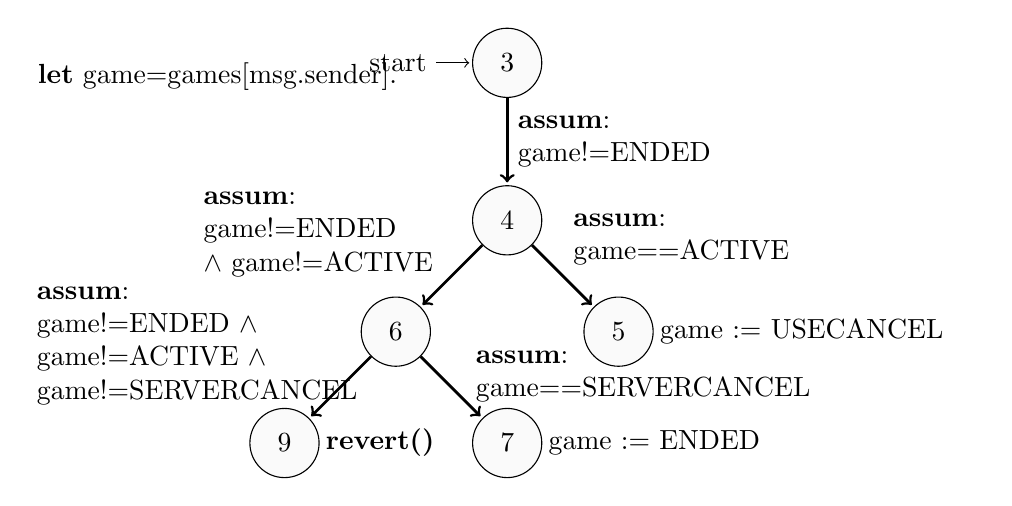
\begin{tikzpicture}[shorten >=1pt,node distance=2cm,auto]
	\tikzstyle{every state}=[fill={rgb:black,1;white,50}]
	\node[state,initial] (q0) {$3$};
	\node[state] (q1) [below of=q0] {$4$};
	\node[state] (q2) [below right of=q1] {$5$};
	\node[state] (q3) [below left of=q1] {$6$};
	\node[state] (q4) [below right of=q3] {$7$};
	\node[state] (q5) [below left of=q3] {$9$};
	
	\node[text width=4cm, xshift=15pt] (line5) [right of=q2] {game := USECANCEL};
	\node[text width=4cm, xshift=15pt] (line7) [right of=q4] {game := ENDED};
	\node[text width=4cm, xshift=15pt] (line7) [right of=q5] {\textbf{revert()}};
		
	\path[->, line width=1pt] (q0) edge node[text width=2cm] {\textbf{assum}: game!=ENDED} (q1) 
							  (q1) edge node[text width=2cm] {\textbf{assum}: game==ACTIVE} (q2) 
							  (q1) edge node[text width=3cm, yshift=15pt, xshift=10pt, left of=q1] {\textbf{assum}: game!=ENDED $\land$ game!=ACTIVE} (q3) 
  							  (q3) edge node[text width=3cm, xshift=5pt, yshift=-9pt] {\textbf{assum}: game==SERVERCANCEL} (q4) 
  							  (q3) edge node[text width=3cm, yshift=15pt, xshift=-10pt, left of=q1] {\textbf{assum}: game!=ENDED $\land$ game!=ACTIVE $\land$ game!=SERVERCANCEL} (q5) 
	 ;
 	\node (label) [yshift=-5pt, xshift=-70pt, above of=q1, text width=7cm] { \textbf{let} game=games[msg.sender]. };			  
\end{tikzpicture}
}
\end{subfigure}


\caption{The control flow graph of Dicether's \textit{userCancelGame}.}
\label{fig: abstractionDicetherFunction}
\end{figure}